\documentclass[margin=1pt]{standalone}

\usepackage{tikz}

\begin{document}
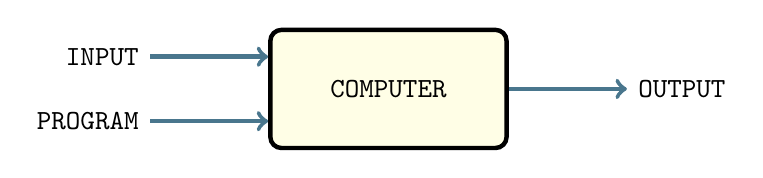
\begin{tikzpicture}[
    ultra thick,
    arr/.style={ultra thick, cyan!50!black},
    lab/.style={font=\ttfamily, black},
  ]
  \node[
    rectangle, draw =black, fill =yellow!10,
    minimum width=3cm, minimum height=1.5cm,
    rounded corners,
  ] (comp) at (0,0) {\texttt{COMPUTER}};

  \draw[arr, to-] (comp.165) -- ++ (-1.5,0) node[lab, left] {INPUT};
  \draw[arr, to-] (comp.195) -- ++ (-1.5,0) node[lab, left] {PROGRAM};
  \draw[arr, -to] (comp.0) -- ++ (1.5,0) node[lab, right] {OUTPUT};
\end{tikzpicture}
\end{document}
